%%%%%%%%%%%%%%%%%%%%%%%%%%%%%%%%%%%%%%%%
%                                      %
% Athanassios Protopapas, October 2005 %
% Mini-example for using apa.cls       %
%                                      %
%%%%%%%%%%%%%%%%%%%%%%%%%%%%%%%%%%%%%%%%

\documentclass{apa}
\usepackage[cp1250]{inputenc}
\usepackage{times,epsfig}



\title{Web semantization}
\author{Peter Vojt�, Jan D�dek, Alan Eckhardt, Leo Galambo�}
\affiliation{Department of software engineering, Faculty of Mathematics and Physics, Charles University\\
Institute of Computer Science, Academy of Sciences of the Czech Republic }

\abstract{Abstract.}

\acknowledgements{.}

\shorttitle{Web semantization}
\rightheader{Web semantization}
\leftheader{P.\ Vojt�}

\begin{document}
\maketitle                            
Introduction.

\section{Problem} 
\subsection{Searching for a used car}
In our work for web semantization, we started with an illustrative example of a user buying a used car. She wants to get a reliable car with a small consumption. The car should also have as many airbags as possible. There are lot of other attributes of a car that may or may not be significant for the user. There are also attributes of the seller of the car, such as the price of the car, the confidence of the seller or the geographical position of the shop, where the car is parked.\par
In the current state of Web, our user has to access several (many) web pages to find a car she would really like. She can have no assurance that she have found the best one; she maybe missed one seller or did not look on the right page. Web pages of sellers also often do not present all necessary information about the cars they offer. She have to go to e.g. the car manufacturer's page, where the given car model is described.\par


	\begin{figure}
		    \begin{center}
		          	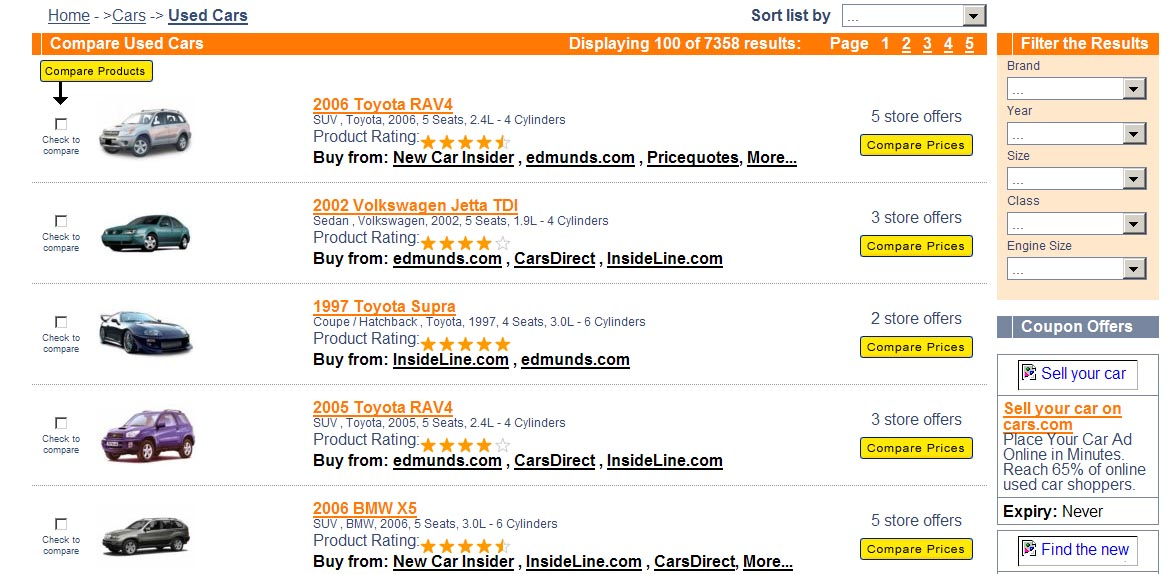
\includegraphics[scale=0.4]{screenshots/activeshopper.jpg}		          
		    \end{center}
		    \caption{A screenshot from Active shopper website}
		    \label{fig:activeShopper}
  \end{figure}
  
There exists pages that gather information about cars or other goods (http://www.activeshopper.com, see Figure \ref{fig:activeShopper}). These pages are often only a list of names of goods with their price and sellers without any further information about the product. For making use of them, the user have to first find what type of car she wants and then find the lowest price. Even then she might not be satisfied - the seller might be in other region or be unreliable etc. The price is not the only criteria.

	\begin{figure}
		    \begin{center}
		          	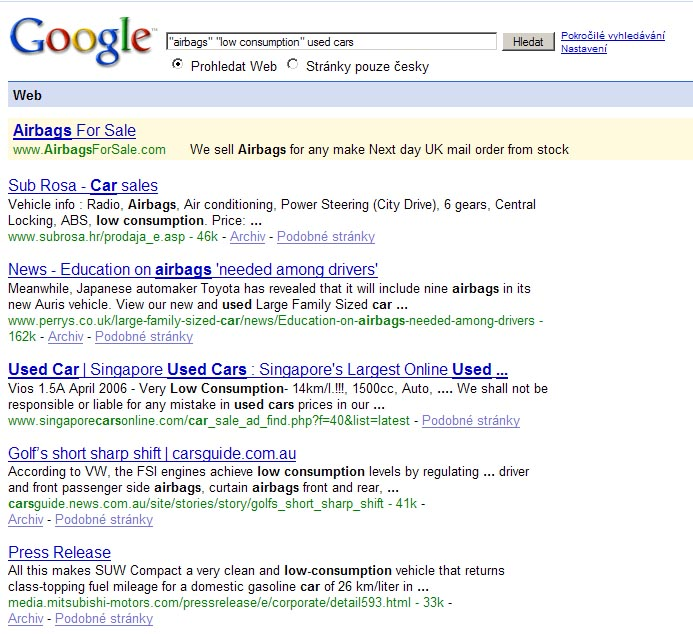
\includegraphics[scale=0.4]{screenshots/googleSearch.jpg}		          
		    \end{center}
		    \caption{Results from keyword search from Google.com}
		    \label{fig:googleSearch}
  \end{figure}
  
\subsubsection{Keyword search limitations}
If the user wanted to use Google \cite{google} (see Figure \ref{fig:googleSearch}) to find a good car, she would not be any more successful. Using keywords is a good method when searching some information about cars, but not so much when you search a car with some properties. Using keywords such as "airbags" or "low consumption" may lead to a better results, but the search on the web page is necessary.

\subsubsection{Car search in a semantized web}
Let's assume that web have gone a little bit semantized - some information is stored on web pages in a machine-readable form, there are distributed lists of such pages, some ontologies exists and are widely used.\par
In this web, our user would have a virtual agent that will search the car for her. She only has to express her preferences in terms of an ontology that describes cars and their sellers. The agent will then search for pages that contains information about cars. It can decide, which car is more appropriate for the user based on the properties of cars and their sellers. It has to combine information about both to an overall degree of preference. It provides the user with this degree as well as other information about the car. She can rectify the agent by rating his results. The agent refines his criteria on cars and on sellers this way.\par
In this scenario, the user does not need to access any page at all. She can, if she is interested in a particular offer, to find out more detail about it. The agent do all the crawling work and present the user only with the offers she may find interesting.\par
The problem is that now the web is not semantized at all. In this paper, we address some of the aspects:
\begin{enumerate}
\item How to extract information from current web pages,
\item How to store this information in a machine readable form,
\item	How to combine this information into a preference degree.
\item {\bf(A dal, jeste neco?)}
\end{enumerate}



\subsection{A gap between Web of today and the Semantic Web}
There are two extreme positions in web development and hence also in research and development on web technologies. One is, "�the Semantic Web is dead and let us concentrate on tagging, mashups, AJAX, etc�". Another extreme position is to study only the Semantic Web without any connection with the Web of today (see panel at ISWC07 "�the biggest fallacy of SW�").  As emphasized  by our title "Web Semantization", we understand the grand vision of the Semantic Web \cite{biblio:2001-Berners-Lee-SemanticWeb} rather as a process of making the Web of today more semantic, i.e. to make it more machine understandable and/or processable. We think that we can already start filling the gap between Web of today and the Semantic Web, see section~\ref{sec:idea_semantization} \textbf{nefunguje!?} for more details.


\section{My Idea}

\subsection{Semantic search engine for software agents} \label{sec:idea_semantization}

There exist many tools for extraction of information form web pages \textbf{doplnit citace} and we are also working on development of some of them (see following sections). We would like to use these tools to produce semantic annotations of web pages and we would like to make these annotations accessible for other software agents. So we propose making a semantic search engine denoted to software gents.

Making such search engine cold help to arch over %preklenout :-)
the gap between Web of today and the Semantic Web. We can expect that performance and quality of extraction tools will improve in near future and so the semantics provided by the search engine will be better and better. Authors of web pages have the possibility to support semantic content on their pages and this way they can improve contemporary Web and indeed the search engine. Success of such search engine would motivate both: (1) authors of web pages to include semantic content and (2) authors of software agents to exploit the semantic content.

\subsection{Third party annotations}

\textbf{Uvedeni neurcitosti, konfidence jednotliv�ch anotaci}

\textbf{Uvedeni paramatru extraktoru, ktery produkoval jednoltive anotace --- trenovaci data, jmeno experta ktery vytvoril extrakcni pravidla, identifikace extrakcni ontologie}


\subsection{Subsection1}
\subsubsection{Ontologies}
\subsubsection{Agent proposal}
- Use of uncertainty -
	- uncertainty of WIE (epistemic)
		- name of the tool, train data, ontology used
		- feedback from the user - alter relevance of the tool on the page used
	
\subsubsection{Web search/LG}
\subsubsection{Decathlon - conflicting objectives/AE}
One of the aspects our proposed agent should be able to do is to compare different objects based on their attributes. We call this "decathlon effect", or in economy terminology "conflicting objectives". The problem is that cars have several attributes, such as number of airbags, reliability, maximum speed etc. The user have some preferences on these attributes, she wants many airbags, lower maximum speed, high reliability... These preferences are called objectives. We can use fuzzy logic notation and to each attribute $A_i$ associate its fuzzy function $f_i:D_{A_i}\rightarrow[0,1]$\par, which normalize the domain of the attribute.
Some of these objectives are conflicting e.g. wanting high maximum speed and low consumption. There is no clear winner, some of the cars may be incomparable - Audi TT has high speed but high consumption, on the other hand Ford Focus may have lower speed but also lower consumption. Regarding two objectives "high speed" and "low consumption", these two cars are incomparable.\par
This undecidability is solved by an aggregation function, often denoted by @. This function takes preference on attributes and combines them into one global score of the whole object (car). In this way, the agent can order all cars by their score. The aggregation function may be a weighted average, for example $@(Speed,Consumption)=(3*Speed+1*Consumption)/4$, where $Speed$ and $Consumption$ are the degrees to which the car satisfies a criteria.\par
{\bf//TODO - co z toho hodit do related work?}\\
This problem is widely addressed in the database engine field. Among most important are \cite{Fagin},\cite{Ilyas}. These works concentrate to the problem, how to get first k objects as fast as possible. They often deal only with a database environment, where data is stored inside one database. Different sources are permitted in \cite{Fagin}. They have to obey certain limitations, which are not strict and can be overcome. This enable the distributed use - obtaining data from other web sources like web services.

\subsubsection{Linguistic}

\subsection{Details of my idea}

\subsection{Web search/LG}
\subsection{Top-k search}
Our top-k search is based on the model from \cite{Fagin}. This model is based on a two-step approach. In the first step, $N$ lists $L_i$ of objects are created, where $N$ is the number of attributes. Each list $L_i$ is ordered by the preference by the preference on the attribute $A_i$. In our example, in the list $L_Consumption$ ordered by the preference on consumption, cars with low consumption would be on the top of $L_Consumption$ and cars with high consumption would be on the bottom of $L_Consumption$. Each list has to be able to return the top element on the list in a sequential way. The algorithm proceeds from the top to the bottom of each list.\par
Lists consist basically of tuples $(Car, Degree of preference of attribute value)$, e.g. for list $L_Consumption$ one tuples may be $(Audi TT, 0.2)$. This tuple says that car Audi TT has preference of its consumption 0.2, in other words, it has not very good consumption. The algorithm then combines the preference degrees obtained from each list into the global score of the car. This step corresponds to the aggregation function.\par


	\begin{figure}
		    \begin{center}
		          	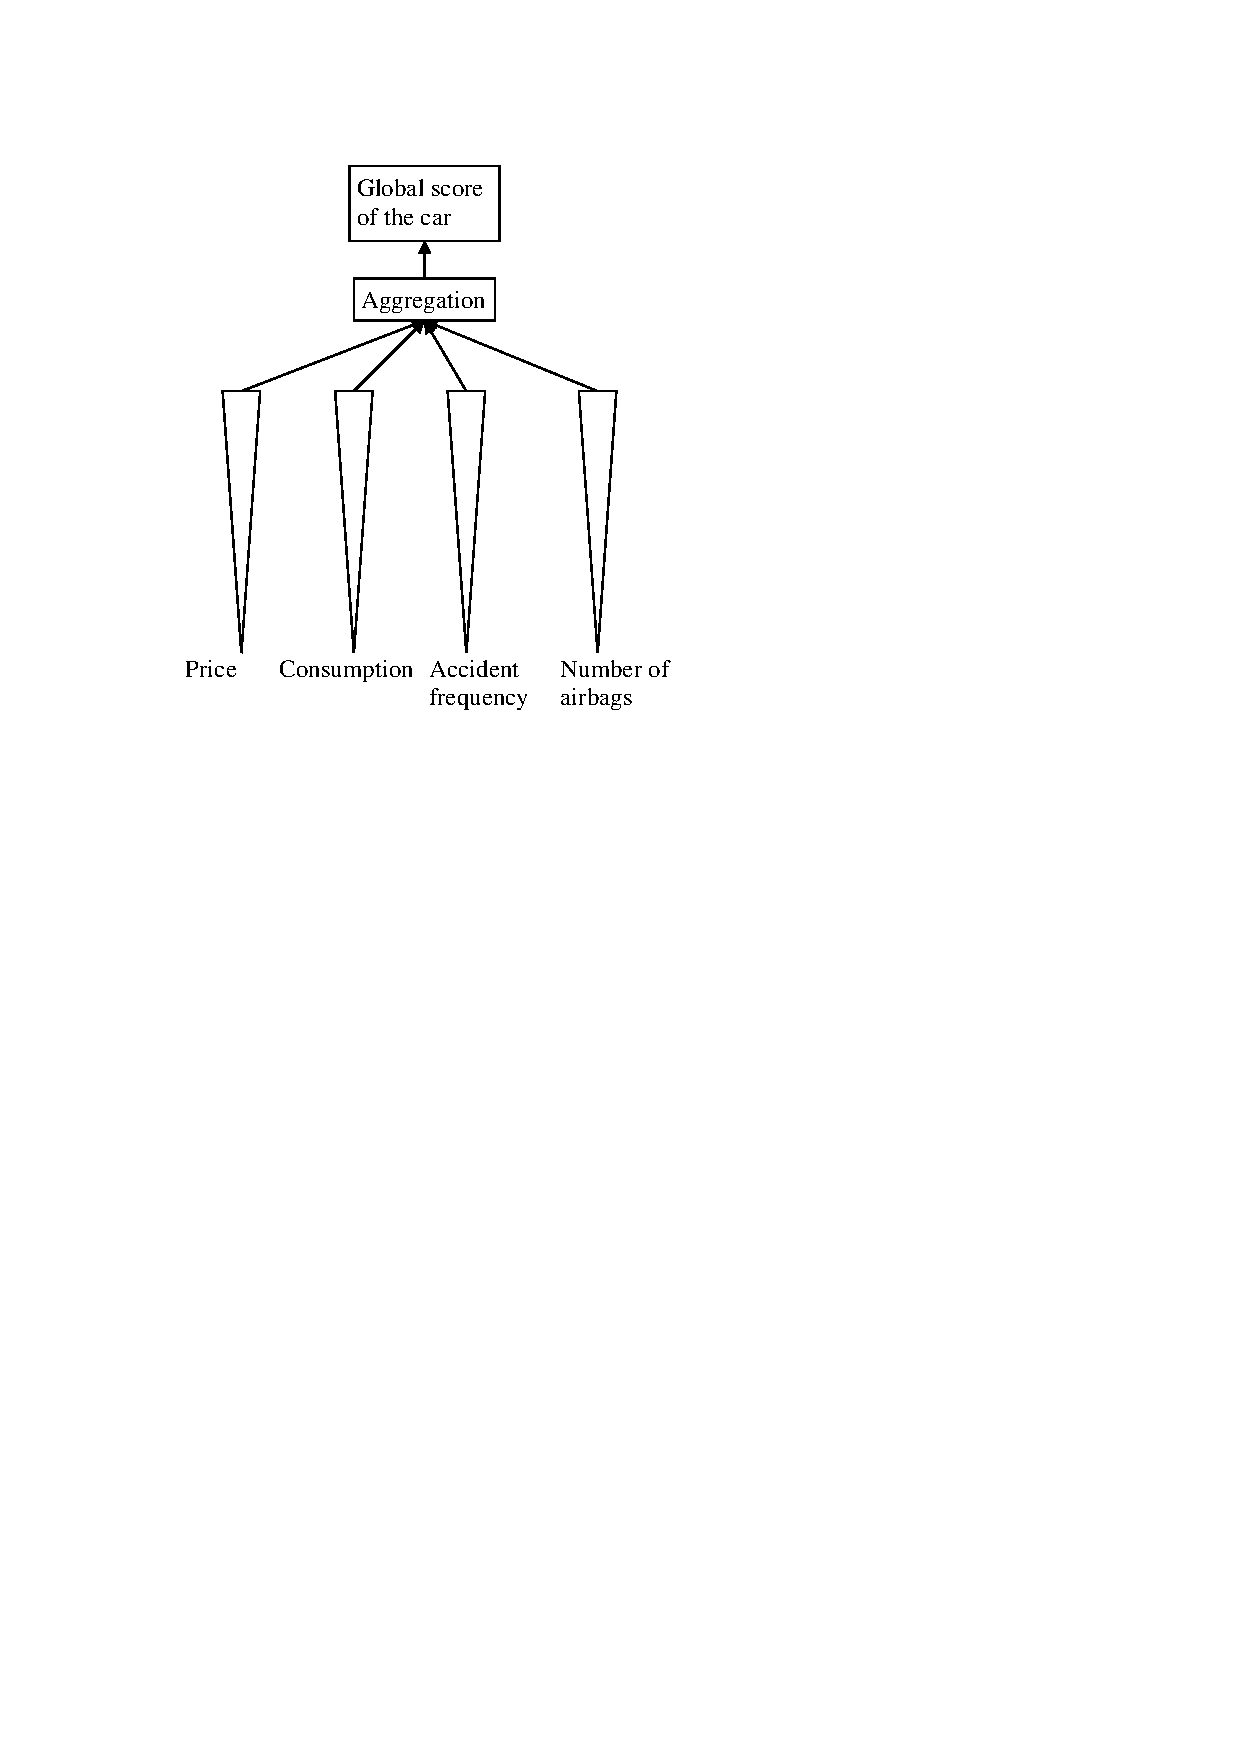
\includegraphics[scale=0.4]{figures/topk.pdf}		          
		    \end{center}
		    \caption{Data flow in a top-k system}
		    \label{fig:topk}
  \end{figure}
  
One big advantage of this approach is that the lists can be generated in different places. This allows computation over distributed sources of data. This is ideal for our situation, when the agent has to combined preferences on data which are gathered from different web sites, maybe using different annotation software. \par

\subsubsection{Certainty about the global ratings}
The agent may use information about uncertainty when using 3-rd party annotations that provides this information. Annotations are not 100\% accurate and some mistakes can be introduced during the annotation process. Information about how certain is annotated information can be stored in the ontology describing these annotations. This degree of certainty then can be used to compute the overall certainty about the final rating. These certainties can be combined in the same way as the preferences. E.g. when information about price of a car is certain on 50\% and the rest on 99\%, we can say that the certainty about the global rating of this particular car is 60\%, because price is very important. On the other hand, certainty about the presence of radio is not so important, so the degree of certainty play little role.\par



\subsection{Web information extraction}
- Learning of tools for WIE 
	- user assisted
		- qualified user
		- unqualified user
	- data
		- text, tables
		- pictures, video, flash scripts
	
\subsection{Experiment/JD+AE}
In our experiment, we tried to integrate information about car offers and information about accident frequency of particular car marks. We used Vidome software \cite{MaruscakDiplomka} for gathering information about cars and a combined linguistic/ILP approach for accident frequencies. We gathered different attributes about offers - the attribute of the car and the reliability of the car manufacturer. Both pieces of information may be important for the user. There is a lot more things that can be gathered from the web about cars - we could analyze blogs about cars, comments on photographs of cars, police reports, cars tuning etc. All these pages can provide some valuable information about cars.
\subsubsection{Web page analysis}
First part was using \cite{MaruscakDiplomka} on the web pages of used car offers.

\subsubsection{Analysis of firemen reports}
We wanted to analyze the frequency of accidents for different car marks. For this, we used information about car accidents published by firemen. These reports are written in natural language (Czech) without any annotation. These reports were analyzed by a linguistic software, which analyze the structure of sentences. Then, we have manually tagged sentences that talks about a number of injuried and some that do not. This was input for Inductive Logic Programming software, Progol.\par
We tagged about 27 sentences as positive and 31 as negative in the train set and 10 positive and  5 negative in the evaluation set. - 73,33\% uspesnost
We tagged about 15 sentences as positive and 1 as negative in the train set and 21 positive and  34 negative in the evaluation set. - 87,50\% uspesnost


\section{Related work}

\section{Conclusion and future work}
\bibliography{citace}

\end{document}
